%!TEX root = ../ShajiS_RnDReport.tex
\documentclass[../ShajiS_RnDReport.tex]{subfiles}

\begin{document}
\section{Introduction}
\label{sec:introduction}

\Glspl{vlm} combine \gls{cv} and \gls{nlp} capabilities in a single neural network. These models can process images and text together, enabling tasks like image classification, image captioning, object detection, and applications like multimodal retrieval - where images are matched with their textual descriptions~\cite{Bordes2024}. While traditional computer vision models are trained for specific tasks like object detection or image classification, vision-language foundation models learn a broader understanding of visual and textual information through pre-training on large-scale web datasets~\cite{Radford2021}. This general understanding allows them to handle new tasks without extensive task-specific training, similar to how \glspl{llm} can be adapted without fine-tuning to different textual tasks~\cite{Liu2023}.

% \begin{figure}[ht]
%     \centering
%     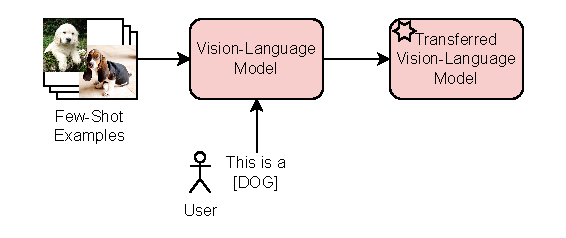
\includegraphics[width=\linewidth]{figures/few-shot-transfer.pdf}
%     \caption{A diagram showing the few-shot transfer process. Each example and its corresponding label is shown to the model. The star denotes that the model has been transferred to a task with examples in-context. The color red denotes that the model is still large and compute-intensive.}
%     \label{fig:few-shot-transfer}
% \end{figure}

\subsection{Motivation}
\label{sec:introduction:motivation}
% Describe the context of your work and the motivation for it.

The standard approach to transferring models to novel tasks is fine-tuning -- a process that adjusts the model's parameters using task-specific training data. However, fine-tuning requires significant computational resources and labeled data, and can also induce catastrophic forgetting~\cite{French1999}. The inherent generalizability of foundation models suggests a more streamlined alternative: \glspl{vlm} can perhaps be adapted to new tasks by showing them a few examples of the task or describing it in natural language~\cite{Tsimpoukelli2021,Li2023}. This approach, known as few-shot learning or few-shot transfer~\cite{Brown2020}, could make such models more practical for real-world applications.

\subsection{Problem Statement}
\label{sec:introduction:problem_statement}
% Describe the problem you are addressing in the work.

Creating labeled datasets for computer vision tasks is generally time-consuming and expensive~\cite{Deng2009}. Our research investigates whether vision-language models can help automate this process by automatically generating labels (which we call pseudolabels) for unlabeled datasets. While these models are powerful, their computational requirements make them impractical for direct use in resource-constrained environments like robots. Therefore, we explore using these models to generate pseudolabels for task-specific datasets, which can then be used to train smaller, more efficient models suitable for deployment.

\begin{figure}[ht]
    \centering
    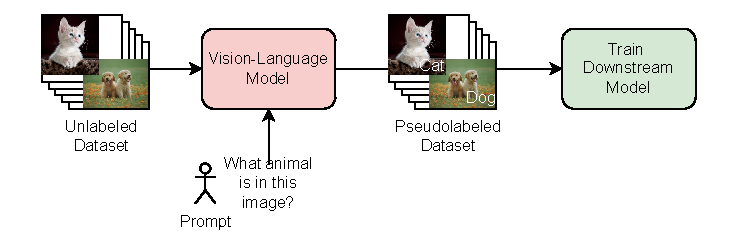
\includegraphics[width=\linewidth]{figures/vlm_transfer_downstream.pdf}
    \caption{Using a vision-language model to generate pseudolabels for a downstream task, which are then used to train a downstream model. In-context examples may be provided to the model (few-shot transfer) or the task may be described in natural language (zero-shot transfer). The color red denotes that the model is large and compute-intensive, while green denotes a smaller, more efficient model.}
    \label{fig:vlm-transfer-downstream}
\end{figure}

\subsection{Proposed Approach}
\label{sec:introduction:proposed_approach}
% Write a short summary of your proposed approach.

We evaluate the effectiveness of vision-language models at generating accurate pseudolabels under different experimental transfer conditions. Our experiments cover both common visual tasks that these models might have encountered during pre-training and specialized tasks they likely haven't seen during pre-training. This helps us understand when and how these models can be reliably transferred for automatic dataset labeling, and whether pre-existing knowledge of the task from pre-training is necessary for reliable transfer.

Our research focuses on three key aspects: 
\begin{enumerate}
    \item How the number of examples shown to the model (few-shot transfer) affects generated pseudolabel quality compared to simply describing the task (zero-shot transfer).
    \item The computational requirements for practical application of these models in few-shot scenarios.
    \item The effectiveness of the smaller downstream models trained on the generated pseudolabels.
\end{enumerate}

\subsection{Report Structure}
\label{sec:introduction:report_structure}
The remainder of this report is organized as follows:

\begin{itemize}
    \item Section~\ref{sec:related_work} reviews relevant literature across four areas: vision-language model development, transfer learning and adaptation techniques, applications and datasets, and current limitations in the field.
    
    \item Section~\ref{sec:methodology} describes our experimental methodology, including the datasets used (CIFAR-10 and the Seven-Point Checklist Dermatology Datasets), model selection criteria, prompting strategies, and downstream model training approach.
    
    \item Section~\ref{sec:evaluation} presents our experimental results, analyzing VLM performance on both general (CIFAR-10 Dataset) and specialized (Seven-Point Checklist Dermatology Dataset) tasks, resource requirements, and downstream model effectiveness.
    
    \item Section~\ref{sec:conclusions} summarizes our key findings, discusses their implications for practical applications, and outlines directions for future research.
\end{itemize}

\end{document}
